\documentclass[12pt,letterpaper,titlepage]{report}
\usepackage{fontspec}
\defaultfontfeatures{Mapping=tex-text}
\usepackage{xunicode}
\usepackage{xltxtra}
\usepackage{enumitem}
\setmainfont{Times New Roman}
\usepackage{amsmath}
\usepackage{amsfonts}
\usepackage{amssymb}
\usepackage{multicol}
\usepackage{paracol}
\usepackage{graphicx}
\graphicspath{{img/}}
\usepackage{karnaugh-map}
\usepackage[margin=0.65in]{geometry}
\author{Jacob Abel}
\title{%
	Homework 6
	\\\large ECE2504 CRN:82729
}

\begin{document}
\maketitle
\begin{raggedright}
\raggedcolumns
\paragraph{Question 1:}
(5 pts) Design a 5x32 decoder using 2x4 decoders with enable and one 3x8 decoder.
\begin{center}
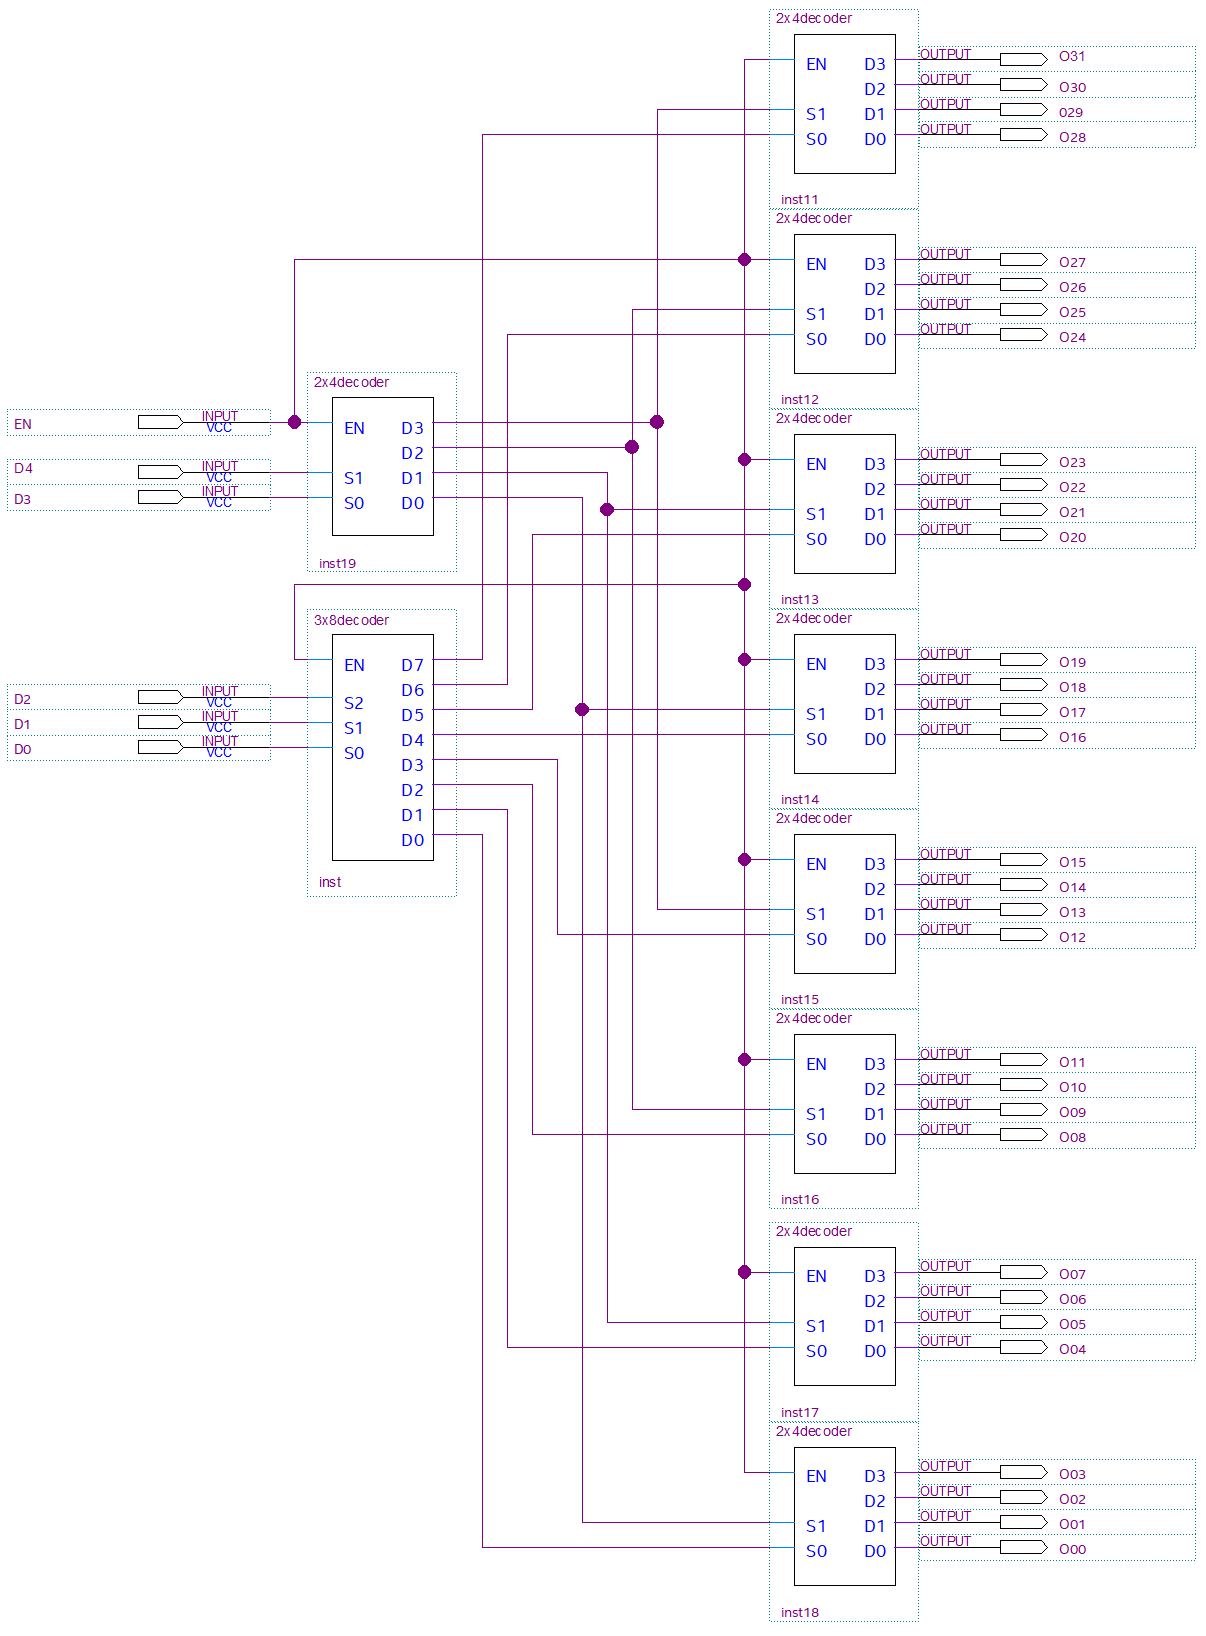
\includegraphics[width=\textwidth,height=0.9\textheight,keepaspectratio=true]{hw6p1}
\end{center}
\clearpage

\paragraph{Question 2:}
(6 pts) Design a 3‐input priority encoder with inputs and outputs as in the table below. 

\begin{paracol}{2}
\begin{center}
\begin{tabular}{|c|c|c||c|c|c|}\hline 
\multicolumn{3}{|c||}{Inputs}&\multicolumn{3}{|c|}{Outputs} \\\hline \hline
$D_2$ & $D_1$ & $D_0$ & $A_1$ & $A_0$ & $V$ \\\hline
0 & 0 & 0 & X & X & 0 \\ 
0 & 0 & 1 & 0 & 0 & 1 \\ 
X & 1 & X & 0 & 1 & 1 \\ 
1 & 0 & X & 1 & 0 & 1 \\\hline
\end{tabular} 
\end{center}
\switchcolumn
\begin{align*}
A_1 =& D_2\overline{D_1}\\
A_0 =& D_1\\
V   =& D_2+D_1+D_0\\
\end{align*}
\end{paracol}
\begin{center}
\includegraphics[width=\textwidth,height=0.9\textheight,keepaspectratio=true]{hw6p2}
\end{center}

\paragraph{Question 3:}
(8 pts) For the electronic game control circuit designed in HW5:Q3, implement a, b, c, and d using a 3x8 decoder and external OR gates. (Assume a maximum of 4 inputs for each gate.) 
\setcolumnwidth{0.3\textwidth, 0.7\textwidth}
\begin{paracol}{2}
\begin{center}
\def\arraystretch{1.1}
\begin{tabular}{|c c c| c c c c |}\hline
$X_2$ & $X_1$ & $X_0$ & a & b & c & d \\\hline
            0 & 0 & 0 & 0 & 0 & 0 & 0 \\\hline
            0 & 0 & 1 & 0 & 0 & 0 & 1 \\\hline
            0 & 1 & 0 & 1 & 0 & 0 & 0 \\\hline
            0 & 1 & 1 & 1 & 0 & 0 & 1 \\\hline
            1 & 0 & 0 & 1 & 1 & 0 & 0 \\\hline
            1 & 0 & 1 & 1 & 1 & 0 & 1 \\\hline
            1 & 1 & 0 & 1 & 1 & 1 & 0 \\\hline
            1 & 1 & 1 & 0 & 0 & 0 & 0 \\\hline
\end{tabular}
\end{center}
\switchcolumn
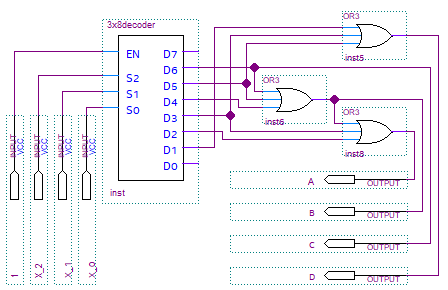
\includegraphics[width=0.9\columnwidth, height=\textheight, keepaspectratio=true]{hw6p3}
\end{paracol}


\clearpage
\paragraph{Question 4:}
(6 pts) Implement the Boolean function $F(A,B,C,D) = \Sigma(0,7,8,9,10,13,14,15)$
\begin{enumerate} [label=\alph*)]
\item with an 8x1 multiplexer and a single inverter with variable D as its input.
\setcolumnwidth{0.35\textwidth, 0.65\textwidth}
\begin{paracol}{2}
\def\arraystretch{1.1} 
\begin{tabular}{|cccc|cc|}\hline 
A & B & C & D & F& \\ \hline
0 & 0 & 0 & 0 & 1& \\ 
0 & 0 & 0 & 1 & 0&$F=\overline{D}$ \\ \hline
0 & 0 & 1 & 0 & 0& \\ 
0 & 0 & 1 & 1 & 0&$F=0$ \\ \hline
0 & 1 & 0 & 0 & 0& \\ 
0 & 1 & 0 & 1 & 0&$F=0$ \\ \hline 
0 & 1 & 1 & 0 & 0& \\  
0 & 1 & 1 & 1 & 1&$F=D$ \\ \hline
1 & 0 & 0 & 0 & 1& \\ 
1 & 0 & 0 & 1 & 1&$F=1$ \\ \hline 
1 & 0 & 1 & 0 & 1& \\  
1 & 0 & 1 & 1 & 0&$F=\overline{D}$ \\ \hline 
1 & 1 & 0 & 0 & 0& \\  
1 & 1 & 0 & 1 & 1&$F=D$ \\ \hline
1 & 1 & 1 & 0 & 1& \\ 
1 & 1 & 1 & 1 & 1&$F=1$ \\ \hline
\end{tabular} 
\switchcolumn
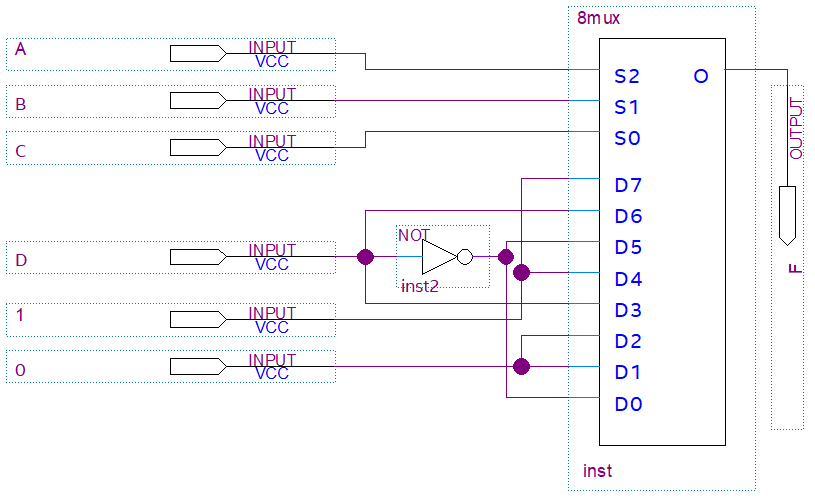
\includegraphics[width=0.9\columnwidth, height=\textheight, keepaspectratio=true]{hw6p4a}
\end{paracol}
\item with a 4x1 multiplexer and 2-input logic gates with variables C and D as input.
\setcolumnwidth{0.4\textwidth, 0.6\textwidth}
\begin{paracol}{2}
\def\arraystretch{1.1} 
\begin{tabular}{|cccc|cc|}\hline 
A & B & C & D & F& \\ \hline
0 & 0 & 0 & 0 & 1& \\ 
0 & 0 & 0 & 1 & 0& \\ 
0 & 0 & 1 & 0 & 0& \\ 
0 & 0 & 1 & 1 & 0&$F=\overline{C+D}$ \\ \hline
0 & 1 & 0 & 0 & 0& \\ 
0 & 1 & 0 & 1 & 0& \\  
0 & 1 & 1 & 0 & 0& \\  
0 & 1 & 1 & 1 & 1&$F=CD$ \\ \hline
1 & 0 & 0 & 0 & 1& \\ 
1 & 0 & 0 & 1 & 1& \\  
1 & 0 & 1 & 0 & 1& \\  
1 & 0 & 1 & 1 & 0&$F=\overline{CD}$ \\ \hline 
1 & 1 & 0 & 0 & 0& \\  
1 & 1 & 0 & 1 & 1& \\ 
1 & 1 & 1 & 0 & 1& \\ 
1 & 1 & 1 & 1 & 1&$F=C+D$ \\ \hline
\end{tabular} 
\switchcolumn
\includegraphics[width=0.9\columnwidth, height=\textheight, keepaspectratio=true]{hw6p4b}
\end{paracol}
\end{enumerate}


\clearpage
\paragraph{Question 5:}
(4 pts) define the following in your own words 
\begin{enumerate} [label=\alph*)]
\item Decoder: Outputs a 1-value to the pin specified by the input. i.e. $I=011 \implies O=00010000$ 
\item Encoder: Outputs the number of the pin supplying a 1-value. i.e. $I=00010000 \implies O=011$ 
\item Multiplexer Outputs the state of the pin specified by the selection pins. i.e. $I=0101, S=01 \implies O=1$
\item Demultiplexer Outputs the input state to the pin specified by the selection pins. i.e. $I=1, S=10 \implies O=0010$
\end{enumerate}

\vspace{\fill}
\noindent
GRADING SCALE
\medskip

Total: 29 pts
\bigskip

\def\arraystretch{1.5} 
\begin{tabular}{ | l | c | c | c | c | c | c | c | c | } \hline
Pts          & 0  & 3  & 7  & 11 & 15 & 18 & 22 & 25     \\\hline
Letter Grade & D- & D  & C- & C  & B- & B  & A- & A      \\\hline
\end{tabular}
\end{raggedright}
\end{document}